% ============================================================================
%  Concept Paper - Datathon RISTEK Fasilkom UI 2026 - Tim Rizzz
%  Kompilasi: jalankan pdflatex minimal 2x agar sitasi ter-resolve
%  Tata letak mengikuti NeurIPS 2015: kertas letter, blok teks 5,5 x 9 inci,
%  Times 10pt, satu kolom.
% ============================================================================
\documentclass[10pt,letterpaper]{article}

\usepackage[letterpaper,left=1.5in,right=1.5in,top=1in,bottom=1in]{geometry}
\usepackage{mathptmx}
\usepackage[T1]{fontenc}
\usepackage[utf8]{inputenc}
\usepackage[bahasa]{babel}
\usepackage{graphicx}
\usepackage{float}
\usepackage{booktabs}
\usepackage{caption}
\usepackage{titlesec}
\usepackage{microtype}
\usepackage{enumitem}
\usepackage{xcolor}
\usepackage[hidelinks]{hyperref}

% ---- metadata berkas PDF ----
\hypersetup{
  pdftitle={TATAP: Triase Skrining Dini Autisme Multimodal untuk Layanan Posyandu},
  pdfauthor={Timotius Christopher Patrick Sihombing},
  pdfsubject={AI Product Concept Paper, Datathon RISTEK Fasilkom UI 2026},
  pdfkeywords={autisme, skrining dini, multimodal, late fusion, eye-tracking, Posyandu, SDIDTK},
  pdfcreator={},
  pdfproducer={}
}

% ---- gaya judul bagian ala NeurIPS ----
\titleformat{\section}{\normalfont\large\bfseries}{\thesection}{0.8em}{}
\titleformat{\subsection}{\normalfont\normalsize\bfseries}{\thesubsection}{0.7em}{}
\titlespacing*{\section}{0pt}{0.9ex plus .2ex minus .2ex}{0.6ex plus .1ex}
\titlespacing*{\subsection}{0pt}{0.75ex plus .2ex minus .2ex}{0.4ex plus .1ex}

\captionsetup{font=footnotesize,labelfont=bf,skip=2.5pt}
\renewcommand{\tablename}{Tabel}
\renewcommand{\figurename}{Gambar}
\addto\captionsbahasa{\renewcommand{\refname}{Referensi}}
% ---- paragraf ala NeurIPS: tanpa indentasi, dipisah spasi vertikal ----
\setlength{\parindent}{0pt}
\setlength{\parskip}{0.20em}
\setlength{\textfloatsep}{4pt plus 1pt minus 1pt}
\setlength{\intextsep}{4pt plus 1pt minus 1pt}
\renewcommand{\arraystretch}{1.06}

% ---- identitas tim ----
\newcommand{\produk}{TATAP}

\begin{document}

% ============================== HALAMAN SAMPUL ==============================
% Halaman ini adalah cover page dan tidak dihitung dalam batas 5 halaman.
\thispagestyle{empty}
\vspace*{1.2cm}

\begin{center}
\rule{\textwidth}{1.2pt}\\[0.7em]
{\LARGE\bfseries \produk: Triase Skrining Dini Autisme Multimodal\\[3pt]
untuk Layanan Posyandu\par}
\vspace{0.7em}
\rule{\textwidth}{0.5pt}\\[2em]
{\normalsize
\begin{tabular}{ccc}
\textbf{Timotius C. P. Sihombing} & \textbf{Raphael Angelo A. Purnama} &
\textbf{Aqila Malfa Zahira} \\[2pt]
\texttt{\small timotiuspatrick@gmail.com} &
\texttt{\small raphael.adikara@gmail.com} &
\texttt{\small aqilamalfa@gmail.com}
\end{tabular}\\[8pt]
Fakultas Teknologi Maju dan Multidisiplin\\
Universitas Airlangga\par}
\end{center}

\vfill
\begin{center}
{\small AI Product Concept Paper \textbullet\ Datathon RISTEK Fasilkom UI 2026
\textbullet\ Preliminary Round, University Track\par}
\end{center}

\newpage
\setcounter{page}{1}

% ============================== ABSTRAK ==============================
% Abstrak dihitung sebagai bagian dari 5 halaman isi (konfirmasi panitia).
\begin{center}
\begin{minipage}{\dimexpr\textwidth-1in\relax}
{\centering\large\bfseries Abstrak\par}
\vspace{0.4em}
\small
Autisme paling responsif terhadap intervensi pada usia di bawah tiga tahun, tetapi diagnosis
rata-rata baru terjadi pada usia 56 bulan, sekitar 32 bulan setelah keresahan pertama orang
tua. Hambatannya mencakup keterbatasan instrumen skrining lini pertama serta akses asesmen
objektif yang terpusat dan mahal. Makalah ini mengusulkan \emph{rancangan} \produk, alat
triase skrining multimodal untuk anak 16 sampai 30 bulan yang ditujukan untuk berjalan luring
di tablet Android biasa dan dioperasikan kader Posyandu. Selama anak menonton video dua menit,
kamera dan mikrofon merekam pola pandangan, gerak kepala/wajah, dan vokalisasi; model terpisah
menghasilkan probabilitas terkalibrasi per modalitas, lalu \textit{weighted late fusion} yang
sadar kualitas sinyal menggabungkannya menjadi rekomendasi rujukan beserta laporan yang dapat
dibaca manusia, bukan diagnosis. Bukti empiris saat ini terbatas pada cabang pandangan: pada
547 rekaman scanpath dari 54 anak, ukuran efek mencapai $d = 1{,}69$ dengan ROC-AUC 0,845
pada tingkat anak di bawah evaluasi yang dikelompokkan per partisipan, sementara pembagian
acak per citra menaikkan AUC 0,063. Cabang gerak, suara, dan fusi akan diuji prospektif.
\end{minipage}
\end{center}
\vspace{0.5em}

% ============================== 1 PENDAHULUAN ==============================
\section{Pendahuluan}

\subsection{Jendela intervensi yang secara sistematis terlewat}

\looseness=-1
Gangguan spektrum autisme bersifat menetap seumur hidup, tetapi lintasan perkembangannya dapat
diubah bila intervensi dimulai cukup awal. Uji acak terkendali \textit{Early Start Denver
Model} pada anak 18 sampai 30 bulan mencatat kenaikan skor kognitif 17,6 poin setelah dua
tahun, dibandingkan 7,0 poin pada kelompok pembanding, dengan perubahan terbesar pada anak
termuda \cite{dawson2010}. Persoalannya, sistem yang ada tidak menemukan anak pada rentang
usia itu. Kajian lintas negara melaporkan usia rata-rata diagnosis 55,97 bulan, padahal
keresahan pertama orang tua muncul pada 23,64 bulan \cite{vanttila2022}: jeda 32,33 bulan yang
jatuh persis pada periode ketika intervensi paling berdampak. Ketimpangannya lebih tajam di
negara berpenghasilan rendah dan menengah, tempat 40 persen individu autistik baru
terdiagnosis pada usia sepuluh tahun atau lebih dibandingkan 15 persen di negara berpenghasilan
tinggi. Yang berbeda bukan rata-ratanya, melainkan ekor distribusinya, yaitu anak yang
benar-benar luput dari sistem, dan kelompok itulah sasaran produk kami.

\subsection{Penyaring lini pertama yang bocor}

\looseness=-1
Instrumen skrining autisme yang paling luas dipakai adalah \textit{Modified Checklist for
Autism in Toddlers} (M-CHAT), kuesioner yang diisi orang tua. Validasi pada layanan primer
melaporkan sensitivitas 49,2 persen dengan spesifisitas 94,2 persen dan nilai prediksi positif
28,9 persen \cite{mchat2026}; studi lain pada populasi risiko rendah mencatat nilai prediksi
positif 36 persen \cite{sturner2017}. Angkanya berbeda antar validasi dan populasi, tetapi
arahnya konsisten: sebagian anak autistik lolos dari penyaringan. Nilai prediksi positif yang
rendah tidak berarti hasil positif sia-sia, karena banyak anak tersebut memiliki hambatan
perkembangan lain; namun sebagai penyaring khusus autisme kinerjanya bervariasi menurut jenis
kelamin, usia gestasi, dan bahasa anak, sehingga perlu dilengkapi sinyal objektif yang tidak
bergantung pada ingatan orang tua.

\subsection{Ketimpangan akses di Indonesia}

Indonesia belum memiliki data prevalensi autisme nasional. Angka yang beredar berasal dari
ekstrapolasi negara lain atau studi regional yang metodenya tidak sebanding \cite{pontianak2019},
sementara skrining M-CHAT-R di klinik Jakarta menemukan 3,52 persen anak 16 sampai 30 bulan
berisiko tinggi \cite{paediatrica2020}. Di sisi pasokan, kapasitas asesmen spesialis terbatas,
sehingga menaikkan sensitivitas skrining tanpa memperbaiki kapasitas triase hanya memindahkan
masalah menjadi antrean rujukan.

\looseness=-1
Namun ada aset yang sering diabaikan. Indonesia memiliki 338.881 Posyandu dengan 1.059.466
kader aktif, dan program Stimulasi, Deteksi, dan Intervensi Dini Tumbuh Kembang (SDIDTK) sudah
menjadi program pokok Puskesmas yang menjangkau hampir setiap desa setiap bulan
\cite{kemenkopmk2023}. Masalahnya kapasitas deteksi, bukan jangkauan: studi pemberdayaan kader
menemukan pelaksanaan SDIDTK cenderung berhenti pada penimbangan dan pengukuran tinggi badan
karena kader belum terlatih mendeteksi penyimpangan tumbuh kembang \cite{mardhika2022}. Skala
jaringan itu sekaligus menetapkan ukuran dampak yang realistis: pada satu kabupaten dengan 300
Posyandu, satu perangkat per Posyandu yang dipakai empat jam pada hari layanan bulanan dengan
target Lampiran~C memeriksa sekitar 12 ribu sesi per bulan, sehingga yang membatasi perluasan
adalah kapasitas asesmen lanjutan, bukan jumlah perangkat.

\subsection{Solusi yang diusulkan dan kontribusi}

Kami mengusulkan \produk\ (Tes Atensi Tumbuh-kembang Anak berbasis Pandangan), alat triase
skrining multimodal yang dijalankan kader pada tablet Android biasa. Produk ini tidak
menggantikan asesmen klinis maupun menyaingi ketepatan alat laboratorium; perannya melengkapi
ceklis dengan pengukuran objektif untuk membantu keputusan rujukan pada titik layanan yang
sudah menjangkau seluruh desa. Kontribusinya ada tiga: rancangan triase yang menyesuaikan diri
dengan keterbatasan nyata layanan primer Indonesia, yaitu perangkat murah, operator bukan
klinisi, dan konektivitas tidak menentu; pemodelan yang mengutamakan keterjelasan lewat model
unimodal terpisah dan \textit{late fusion} sehingga kontribusi tiap sinyal dapat diaudit;
serta reimplementasi terkendali yang mengukur seberapa besar protokol evaluasi lazim pada
dataset scanpath publik menaikkan AUC.

% ============================== 2 TINJAUAN PUSTAKA ==============================
\section{Tinjauan Pustaka}

\subsection{Atensi visual sebagai penanda perilaku}

Kelainan pola pandang adalah penanda perilaku autisme yang paling konsisten. Studi
longitudinal pada bayi usia 2 sampai 6 bulan menemukan penurunan fiksasi pada mata yang tidak
terjadi pada bayi yang kemudian berkembang tipikal \cite{jones2013}, dan anak dengan autisme
memandang pola geometris jauh lebih lama dibandingkan adegan sosial \cite{pierce2011}.
Sinyalnya muncul sebelum kemampuan berbahasa berkembang, sehingga dapat diukur pada usia
ketika instrumen berbasis wawancara belum dapat diterapkan.

\subsection{Instrumen dan produk yang tersedia saat ini}

\looseness=-1
M-CHAT dan KPSP murah serta mudah disebar, tetapi bergantung pada laporan manusia
\cite{mardhika2022}. Pada kutub objektif, EarliPoint memperoleh izin FDA 510(k) untuk anak 16
sampai 30 bulan \cite{earlitec2023}, tetapi memerlukan eye-tracker khusus di fasilitas klinis
dengan biaya pemeriksaan 599 dolar Amerika \cite{earlipointfaq}. Pembanding digital terdekat
adalah SenseToKnow, yang memakai kamera tablet untuk mengukur 23 fenotipe perilaku; studi
prospektif pada 475 balita di layanan primer Amerika Serikat melaporkan AUC 0,90, sensitivitas
87,8 persen, dan spesifisitas 80,8 persen \cite{perochon2023}. Temuan itu membuktikan
kelayakan kamera perangkat konsumen. \produk\ mengambil pilihan berbeda: dioperasikan kader
secara luring, memakai stimulus Indonesia, dan menjaga model perilaku tetap terpisah agar
dapat diaudit.

\subsection{Representasi scanpath sebagai citra}

Carette dkk. \cite{carette2019} mengusulkan dasar teknis pekerjaan kami: mengubah rekaman
eye-tracking menjadi citra, dengan lintasan pandangan sebagai garis dan dinamikanya dikodekan
pada kanal warna, yaitu kecepatan, akselerasi, dan \textit{jerk}, sehingga prediksi menjadi
klasifikasi citra. Mereka melaporkan AUC di atas 0,9 dengan jaringan saraf, sementara model
non-neural pada makalah yang sama hanya sekitar 0,7.

\subsection{Analisis kesenjangan}

Kesenjangan yang kami sasar bukan ketepatan, melainkan penerjemahan pengukuran objektif
menjadi sistem yang dapat dioperasikan kader secara luring. Kebaruannya bukan kamera tablet,
melainkan orkestrasi skrining universal berbasis Posyandu, \textit{late fusion} sadar kualitas
yang menahan keputusan ketika satu modalitas gagal, dan laporan per modalitas yang dapat
diaudit; Tabel~\ref{tab:gap} pada Lampiran~E merinci posisinya pada sepuluh dimensi.


% ============================== 3 METODOLOGI ==============================
\section{Metodologi}

\subsection{Konsep produk dan alur penggunaan}

\produk\ dirancang menyatu dengan alur SDIDTK yang sudah berjalan, khususnya pada meja keempat
Posyandu. Sasarannya seluruh anak usia 16 sampai 30 bulan yang hadir pada kunjungan
terjadwal, dengan sesi pada usia 18 dan 24 bulan. Rentang itu berimpit dengan jendela
intervensi paling produktif dan dengan indikasi instrumen objektif yang sudah diterima
regulator \cite{earlitec2023}, sekaligus membuat skor dibandingkan terhadap norma kelompok
umur sempit. Sesi tidak dibatasi pada anak yang positif ceklis, sebab sasarannya justru anak
yang terlewat instrumen berbasis laporan; konsekuensinya waktu per anak dan beban rujukan
menjadi kendala rancangan, bukan detail implementasi.

\looseness=-1
Kader mendudukkan anak di depan tablet pada dudukan sederhana, lalu memutar video adegan
sosial sekitar dua menit yang memancing atensi bergantian antara wajah manusia dan objek
non-sosial. Pada dua penanda waktu tetap, aplikasi meminta pengasuh memanggil nama anak
sehingga respons terhadap nama dan latensi vokal punya titik awal terdefinisi. Kamera depan
dan mikrofon merekam sesi yang sama untuk mengestimasi arah pandang, dinamika kepala/wajah,
dan respons vokal langsung di perangkat. Kader menerima skor risiko dengan kategori tindak
lanjut, ringkasan pola pandangan dalam bahasa sederhana, kualitas tiap modalitas, dan alasan
eksplisit bila sistem menahan keputusan; Lampiran~F menampilkan rancangan tampilannya.
Keputusan akhir tetap pada manusia: sistem tidak menyatakan seorang anak autistik, melainkan
bahwa pola atensinya di luar rentang tipikal sehingga layak dirujuk.

\subsection{Arsitektur sistem}

Gambar~\ref{fig:arsitektur} menunjukkan alur pemrosesan. Kontrol kualitas berlapis: pada
perekaman, aplikasi hanya memeriksa hal yang dapat diketahui sebelum pemodelan, yaitu kamera
dan mikrofon berfungsi, wajah tertangkap, dan pencahayaan memadai. Skor kualitas $q_m$ dan
kalibrasi probabilitas berada di dalam masing-masing cabang, karena keduanya baru terhitung
setelah modalitasnya diproses; yang mengalir ke fusi adalah pasangan $(p_m, q_m)$. Cabang
pandangan digambar rinci karena di sanalah risiko teknis terbesar berada: video wajah harus
melewati deteksi wajah dan mata, koreksi orientasi kepala, estimasi titik pandang layar,
penghalusan temporal, lalu pemetaan area minat sebelum menjadi scanpath yang sebanding dengan
data eye-tracker. Uji kelayakan pada Bagian~\ref{sec:poc} berangkat dari scanpath yang sudah
jadi, sehingga rantai inilah yang belum terbukti dan menjadi isi studi jembatan pada
Lampiran~A. Seluruh tahap berjalan luring.

\begin{figure}[t]
\centering
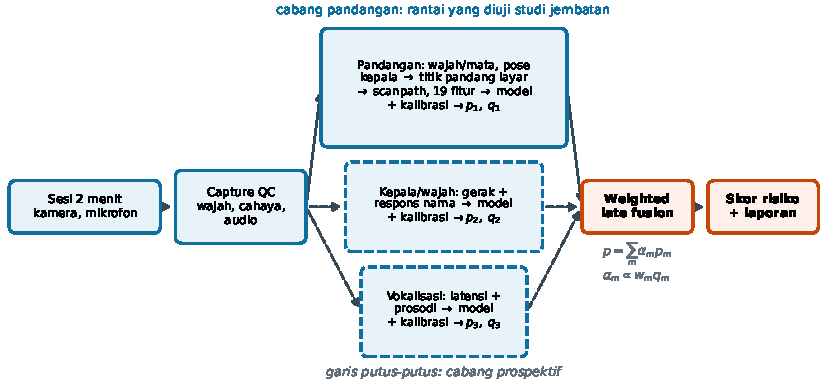
\includegraphics[width=0.76\textwidth]{../../figs/arsitektur.pdf}
\caption{Arsitektur \textit{late fusion} \produk. Blok awal hanya memeriksa mutu perekaman;
setiap cabang memuat pemrosesan, model, kalibrasi, dan skor kualitasnya sendiri lalu mengirim
$(p_m, q_m)$ ke fusi, dan modalitas berkualitas rendah dikeluarkan dengan bobot tersisa
dinormalisasi ulang. Garis putus-putus menandai cabang prospektif yang belum divalidasi.}
\label{fig:arsitektur}
\end{figure}

\subsection{Rencana penggunaan data}

\looseness=-1
Pengembangan memakai tiga lapis data. Lapis pertama, data scanpath publik untuk menguji
premis teknis dan menetapkan garis dasar (Bagian~\ref{sec:poc}). Lapis kedua, studi jembatan
yang merekam anak yang sama dengan eye-tracker laboratorium dan kamera tablet secara bersamaan
untuk mengukur penurunan presisi akibat perpindahan perangkat; kriteria lulusnya ditetapkan
lebih dahulu pada Lampiran~A. Lapis ketiga, data prospektif berpasangan di Posyandu: seluruh
modalitas direkam dari anak dan sesi yang sama, untuk mengalibrasi model, mempelajari bobot,
dan menguji manfaat fusi; fusi pada subjek berbeda tidak dapat ditafsirkan. Acuannya adalah
asesmen perkembangan terstandar dan diagnosis konsensus oleh klinisi yang dibutakan terhadap
keluaran \produk, dengan instrumennya disepakati sebelum pengumpulan data dan kasus yang belum
pasti dipantau ulang, bukan dipaksa masuk salah satu kelas. Seluruh kunjungan dari anak yang
sama ditempatkan pada lipatan yang sama, dan satu lokasi disisihkan sebagai validasi eksternal.
Kohort ini wajib memuat anak dengan hambatan perkembangan non-autisme, seperti keterlambatan
bahasa, gangguan pendengaran, dan keterlambatan umum, sebagai kontrol negatif sulit; tanpa
mereka spesifisitas hanya terukur terhadap anak tipikal.

\subsection{Pendekatan pemodelan}

Setiap modalitas memakai model terpisah. Lintasan pandangan dirender sebagai citra menurut
\cite{carette2019} dan diringkas menjadi 19 fitur tertafsir: cakupan, dispersi, pusat
perhatian, dinamika kanal warna, rasio fiksasi-sakade, dan entropi. Cabang kepala/wajah
merangkum orientasi, stabilitas, dan respons terhadap nama; vokalisasi merangkum latensi,
energi, jeda, dan prosodi, keduanya relatif terhadap dua penanda pemanggilan nama.

\looseness=-1
Probabilitas $p_m$ dikalibrasi lalu digabung sebagai $p=\sum_m\alpha_mp_m$, dengan
$\alpha_m\propto w_mq_m$, kualitas $q_m$, dan bobot nonnegatif $w_m$. Kalibrasi dan
pembelajaran bobot hanya berjalan di lipatan dalam yang dikelompokkan per anak, memakai
\textit{constrained logistic stacking} berpenalti pada prediksi \textit{out-of-fold}; anak dan
lokasi pada lipatan luar tidak pernah ikut mengkalibrasi, sebab tanpa pemisahan ini kenaikan
yang tampak dari fusi dapat berasal dari kebocoran kalibrasi. Rata-rata sama bobot menjadi
garis dasar. Skor kualitas $q_m$ dihitung dari proporsi bingkai dengan wajah terdeteksi,
kestabilan estimasi pandangan, dan rasio sinyal terhadap derau audio. Pembedaannya bukan
teknis semata: kegagalan perekaman, misalnya wajah tak terlihat atau mikrofon tertutup,
menurunkan $q_m$ sehingga modalitasnya dikeluarkan dan bobot dinormalisasi ulang, sedangkan
ketiadaan respons pada rekaman berkualitas baik justru dipertahankan sebagai fitur perilaku.
Menyamakan keduanya membuang sinyal klinis yang paling informatif. Sistem menahan keputusan
dan meminta sesi diulang bila cabang pandangan gagal ambang kualitas, atau bila kurang dari
dua modalitas lolos; layar penahanan menyebut penyebabnya agar kader dapat memperbaikinya.

Fusi hanya diadopsi bila lulus kriteria pada Lampiran~B, yang menuntut perbaikan melampaui
selang kepercayaan, bukan sekadar kenaikan AUC. Evaluasi prospektif membandingkan M-CHAT saja,
pandangan saja, \produk\ multimodal, dan M-CHAT digabung \produk\ pada kohort yang sama:
pertanyaannya apakah \produk\ menemukan anak yang terlewat ceklis atau mengurangi rujukan
yang tidak perlu, tanpa beban di luar kapasitas Puskesmas setempat. Ambang keputusan mengikuti
asimetri biaya skrining: melewatkan anak autistik berarti kehilangan jendela intervensi yang
kerugiannya sering permanen, sedangkan merujuk anak tipikal menimbulkan kecemasan dan biaya
asesmen yang masih dapat dipulihkan. Ambang condong ke sensitivitas tinggi, tetapi angka
finalnya ditetapkan bersama klinisi dari jumlah rujukan per 1.000 anak yang dapat ditangani,
bukan dari optimum statistik.

\subsection{Uji kelayakan awal}
\label{sec:poc}

Untuk menguji premis teknis, kami menganalisis 547 citra scanpath dari 54 anak pada dataset
\cite{carette2019} dengan seluruh evaluasi dikelompokkan per partisipan, sehingga model
selalu diuji pada anak yang belum pernah dilihatnya. Perbedaan antar kelompok muncul dengan
ukuran efek besar pada tingkat partisipan, mencapai $d = 1{,}69$ untuk luas sebaran pandangan
dan $d = 1{,}50$ untuk cakupan area: anak dengan autisme menyapu bidang layar lebih luas dan
merata, sementara anak tipikal memusatkan pandangan pada zona tengah selama 54,0 persen waktu
dibandingkan 43,2 persen.

Karena unit keputusan produk adalah anak, endpoint utama kami adalah AUC tingkat anak dari
regresi logistik, garis dasar yang ditetapkan sebelum hasil dilihat. Setelah probabilitas
\textit{out-of-fold} dirata-ratakan per anak, model itu mencapai ROC-AUC 0,845 (selang
kepercayaan 95 persen 0,730--0,944), dibandingkan 0,753 pada tingkat rekaman. Peringkat antar
model tidak stabil dan \textit{nested GroupKFold} menunjukkan pemilihan model tidak menambah
keunggulan (Lampiran~G), sehingga POC ini tidak menetapkan model produksi dan angkanya
eksploratif.

\looseness=-1
Rata-rata 38,2 persen variasi fitur berada pada tingkat antarpartisipan, sehingga rekaman
berulang dari anak yang sama bukan pengamatan independen. Konsekuensinya terukur: dengan model
dan fitur identik di seluruh protokol, evaluasi acak per citra setelah augmentasi menghasilkan
AUC 0,816 dibandingkan 0,753 pada evaluasi tanpa augmentasi yang dikelompokkan per partisipan
(Gambar~\ref{fig:bukti}c), dan sebagian besar selisih 0,063 itu berasal dari tidak
mengelompokkan per anak (Lampiran~G). Angka ini berlaku untuk konfigurasi kami, bukan koreksi
yang dapat dikurangkan dari hasil orang lain; yang berlaku umum adalah arahnya.

\begin{figure}[t]
\centering
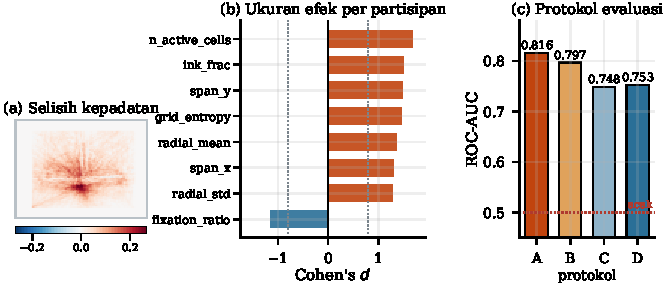
\includegraphics[width=0.66\textwidth]{../../figs/bukti.pdf}
\caption{Bukti kelayakan pada 547 scanpath dari 54 anak. (a) Selisih kepadatan pandangan
rata-rata; merah menandai area yang lebih sering dipandang kelompok autisme. (b) Ukuran efek
antar kelompok pada tingkat partisipan, garis titik menandai ambang efek besar $|d| = 0{,}8$.
(c) AUC dengan model dan fitur identik di bawah empat protokol evaluasi A sampai D, dirinci
pada Lampiran~G; D adalah evaluasi utama kami pada tingkat rekaman.}
\label{fig:bukti}
\end{figure}

Uji ini memvalidasi premis, bukan kesiapan produk: datanya dari anak usia sekolah rata-rata
7,9 tahun, direkam eye-tracker laboratorium pada populasi Prancis, dan titik kerjanya
menegaskan itu. Ambang yang menjaga sensitivitas 90 persen pada tingkat anak memberi 92,3
persen dengan spesifisitas 42,9 persen pada model pra-tetap, sementara model pembanding pada
sensitivitas sama mencapai 57,1 persen meski AUC keduanya nyaris sama: titik kerja jauh lebih
rapuh daripada peringkat model. Pada prevalensi hipotetis 1 persen, nilai prediksi positif
model pra-tetap tinggal 1,6 persen, setara sekitar 62 rujukan per satu kasus benar. Angka itu
bukan ramalan untuk Posyandu, melainkan alasan ambang produksi ditetapkan bersama klinisi
menurut kapasitas rujukan.

\subsection{Rencana pengembangan dan skalabilitas}

Skalabilitas \produk\ bertumpu pada keputusan untuk tidak membangun jaringan distribusi baru:
perangkatnya hanya tablet Android kelas menengah bawah beserta dudukan sederhana, sehingga
biaya per titik layanan berada pada kisaran perangkat konsumen. Kendalanya bukan harga
melainkan waktu: video dua menit menjadi sekitar empat sampai enam menit layanan setelah
penempatan anak, persetujuan, kemungkinan pengulangan, dan penjelasan hasil. Target
Lampiran~C karena itu ditetapkan sebagai median lima menit dengan persentil ke-90 tujuh menit
dan kapasitas sepuluh anak per jam, menyisakan margin untuk pergantian anak dan gangguan
lapangan; bila tidak tercapai, jumlah perangkat yang dinaikkan, bukan durasi sesi yang
dipangkas. Inferensi luring membuat layanan tetap tersedia di wilayah berkonektivitas
terbatas, yang justru wilayah dengan akses spesialis paling rendah.

Pengembangan bertahap: memvalidasi jembatan pengukuran antara eye-tracker dan kamera tablet
sekaligus membangun stimulus versi Indonesia; menjalankan uji coba terbatas dengan target
operasional pada Lampiran~C; lalu memperluas cakupan sambil mengalibrasi ulang terhadap norma
setempat. Cabang vokalisasi dan gerak diuji sebagai penambah nilai, bukan diasumsikan
membantu. Setiap sesi juga menghasilkan catatan risiko skrining terstandar yang menopang
surveilans layanan dan perencanaan kapasitas rujukan; ini melengkapi survei epidemiologis dan
tidak menggantikannya, karena estimasi prevalensi tetap menuntut sampling representatif dan
konfirmasi diagnosis.

% ============================== 4 ETIKA ==============================
\section{Pertimbangan Etis dan Limitasi}

\looseness=-1
Risiko pelabelan ditekan dengan membatasi keluaran pada rekomendasi rujukan, menampilkan
ketidakpastian, dan mensyaratkan persetujuan yang dapat ditarik. Rekaman mentah dienkripsi dan
dihapus otomatis setelah inferensi; hanya fitur dan skor pseudonim yang disinkronkan, dengan
tata kelola dan pelaporan per subkelompok pada Lampiran~D.
Bukti pandangan berasal dari populasi, usia, dan perangkat berbeda sehingga transfer ke
Posyandu masih asumsi; spesifisitas rendah mewajibkan audit beban rujukan, dan bias pandangan
ke letak alat menuntut randomisasi penempatan. Cabang gerak, suara, dan fusi baru boleh
diklaim setelah validasi berpasangan.

% ============================== 5 KESIMPULAN ==============================
\section{Kesimpulan}

\looseness=-1
\produk\ mengusulkan arsitektur pengukuran multimodal untuk tablet Posyandu. Yang
diperjuangkan bukan ketepatan tertinggi, melainkan memindahkan pengukuran objektif ke titik
layanan yang menjangkau hampir setiap desa, agar anak yang luput dari instrumen berbasis
laporan berpeluang dirujuk selagi intervensi paling berdampak. Uji kelayakan menunjukkan
geometri scanpath memuat sinyal berefek besar; titik kerja yang belum stabil menandai sisa
pekerjaan, yaitu studi jembatan lalu kohort prospektif.

% ============================== REFERENSI ==============================
% Bibliografi dimulai di halaman sendiri; tidak dihitung dalam batas 5 halaman.
\newpage
\small
\bibliographystyle{plain}
\begin{thebibliography}{99}

\bibitem{dawson2010}
G.~Dawson, S.~Rogers, J.~Munson, M.~Smith, J.~Winter, J.~Greenson, A.~Donaldson, dan
J.~Varley. Randomized controlled trial of an intervention for toddlers with autism: the
Early Start Denver Model. \textit{Pediatrics}, 125(1):e17--e23, 2010.

\bibitem{vanttila2022}
M.~van~'t~Hof, C.~Tisseur, I.~van~Berckelaer-Onnes, A.~van~Nieuwenhuyzen, A.~M. Daniels,
M.~Deen, H.~W. Hoek, dan W.~A. Ester. Age at autism spectrum disorder diagnosis: a
systematic review and meta-analysis from 2012 to 2019. \textit{Autism}, 25(4):862--873,
2021.

\bibitem{mchat2026}
A.~L. Harper, D.~E. Sarver, dan K.~F. Sly. Validation of the Modified Checklist for
Autism in Toddlers (M-CHAT): a replication study of diagnostic accuracy.
\textit{Journal of Autism and Developmental Disorders}, 2026.
doi:10.1007/s10803-026-07330-3.

\bibitem{sturner2017}
R.~Sturner, B.~Howard, P.~Bergmann, D.~Morrel, L.~Andon, C.~Marks, P.~Rao, dan
M.~Landa. Autism screening with online decision support by primary care pediatricians
aided by M-CHAT/F. \textit{Pediatrics}, 138(3):e20153036, 2016.

\bibitem{pontianak2019}
Fathmawati, L.~Andari, J.~Saimin, D.~F. Damayanti, Z.~Akhmadi, dan E.~D. Septiawan.
Distribution of autistic children in Pontianak, West Kalimantan Province, Indonesia.
\textit{Malaysian Journal of Public Health Medicine}, 23(2):124--130, 2023.
doi:10.37268/mjphm/vol.23/no.2/art.1826.

\bibitem{paediatrica2020}
C.~J. Aditya, J.~K. Dahliana, A.~D. Widodo, dan R.~Sekartini. Autism spectrum disorder
screening in children aged 16--30 months using the Modified Checklist for Autism in
Toddlers-Revised (M-CHAT-R). \textit{Paediatrica Indonesiana}, 61(5):247--252, 2021.
doi:10.14238/pi61.5.2021.247-52.

\bibitem{kemenkopmk2023}
Kementerian Koordinator Bidang Pembangunan Manusia dan Kebudayaan RI. Posyandu miliki
peran penting ciptakan generasi emas Indonesia, 2023.

\bibitem{mardhika2022}
A.~Mardhika, J.~Susanto, E.~Qurniyawati, dan A.~P.~M. Tyas. Empowerment of healthcare
cadres on stimulation of early detection and intervention of growth and development.
\textit{Abdimas Unwahas}, 7(2), 2022. doi:10.26905/abdimas.v7i2.6909.

\bibitem{jones2013}
W.~Jones dan A.~Klin. Attention to eyes is present but in decline in 2--6-month-old
infants later diagnosed with autism. \textit{Nature}, 504(7480):427--431, 2013.

\bibitem{pierce2011}
K.~Pierce, D.~Conant, R.~Hazin, R.~Stoner, dan J.~Desmond. Preference for geometric
patterns early in life as a risk factor for autism. \textit{Archives of General
Psychiatry}, 68(1):101--109, 2011.

\bibitem{earlitec2023}
U.S. Food and Drug Administration. EarliPoint System, 510(k) K213882, 2022; EarliPoint,
510(k) K230337, 2023.

\bibitem{earlipointfaq}
EarliPoint Health. Frequently asked questions. Diakses 2026.

\bibitem{perochon2023}
S.~Perochon, J.~M. Di~Martino, K.~L.~H. Carpenter, S.~Compton, N.~Davis, B.~Eichner,
S.~Espinosa, L.~Franz, P.~R. Krishnappa~Babu, G.~Sapiro, dan G.~Dawson. Early detection
of autism using digital behavioral phenotyping. \textit{Nature Medicine},
29:2489--2497, 2023. doi:10.1038/s41591-023-02574-3.

\bibitem{carette2019}
R.~Carette, M.~Elbattah, F.~Cilia, G.~Dequen, J.-L. Gu\'erin, dan J.~Bosche. Learning to
predict autism spectrum disorder based on the visual patterns of eye-tracking scanpaths.
Dalam \textit{Proceedings of BIOSTEC 2019 (HEALTHINF)}, halaman 103--112, 2019.

\end{thebibliography}

% ============================== LAMPIRAN ==============================
% Lampiran tidak dihitung dalam batas 5 halaman.
\newpage
\normalsize
\section*{Lampiran A. Kriteria go/no-go studi jembatan eye-tracker ke kamera tablet}
\addcontentsline{toc}{section}{Lampiran A}

Studi jembatan merekam anak yang sama dengan eye-tracker laboratorium dan kamera tablet
secara bersamaan; yang diukur adalah kesetaraan pengukuran, bukan akurasi diagnosis. Kriteria
berikut ditetapkan sebelum data dikumpulkan. Nilai di zona tengah tidak menghentikan program,
tetapi mewajibkan satu putaran perbaikan terarah lalu pengukuran ulang pada sampel baru,
bukan penyetelan ulang model terhadap data yang sama. Kegagalan pada satu baris mana pun
menghentikan konfigurasi perangkat atau stimulus yang diuji.

\begin{table}[H]
\centering
\small
\caption{Kriteria kelulusan studi jembatan. Nilai adalah target pengembangan, bukan hasil
yang sudah dicapai.}
\label{tab:gonogo}
\begin{tabular}{@{}p{0.34\textwidth}p{0.20\textwidth}p{0.19\textwidth}p{0.17\textwidth}@{}}
\toprule
\textbf{Indikator} & \textbf{Lulus} & \textbf{Revisi dan uji ulang} & \textbf{Gagal} \\
\midrule
Galat sudut estimasi pandangan (median) & $\leq 3{,}0^\circ$ & $3{,}0^\circ$--$5{,}0^\circ$ & $> 5{,}0^\circ$ \\
Bingkai dengan wajah dan mata terdeteksi & $\geq 85$ persen per sesi & 70--85 persen & $< 70$ persen \\
Kesesuaian fitur webcam vs eye-tracker & ICC $\geq 0{,}75$ pada fitur dispersi & ICC 0,60--0,75 & ICC $< 0{,}60$ \\
Kesesuaian okupansi area minat & selisih $\leq 10$ poin persen & 10--20 poin persen & $> 20$ poin persen \\
Sesi gagal dan perlu diulang & $\leq 10$ persen & 10--25 persen & $> 25$ persen \\
Selisih kualitas antar subkelompok (kacamata, pencahayaan rendah, tipe tablet) & dalam batas dua kriteria di atas & satu kriteria di zona tengah & satu kriteria gagal \\
\bottomrule
\end{tabular}
\end{table}

\section*{Lampiran B. Kriteria penerimaan fusi multimodal}

Fusi hanya menggantikan cabang pandangan bila seluruh kriteria berikut terpenuhi pada
kohort prospektif berpasangan, dengan evaluasi dikelompokkan per anak dan seluruh metrik
dihitung pada unit anak.

\begin{table}[H]
\centering
\small
\caption{Kriteria penerimaan fusi. Perbandingannya selalu terhadap cabang pandangan saja
pada kohort yang sama.}
\label{tab:fusi}
\begin{tabular}{@{}p{0.30\textwidth}p{0.64\textwidth}@{}}
\toprule
\textbf{Dimensi} & \textbf{Ambang penerimaan} \\
\midrule
Sensitivitas & $\geq 90$ persen pada ambang rujukan yang disepakati klinisi \\
Beban rujukan & Rujukan per 1.000 anak tidak lebih tinggi daripada cabang pandangan pada sensitivitas sama \\
Diskriminasi & Kenaikan AUC yang batas bawah selang kepercayaan 95 persennya di atas nol, bukan sekadar rerata lebih tinggi \\
Kalibrasi & \textit{Calibration slope} pada rentang 0,9 sampai 1,1 dan \textit{Brier score} membaik \\
Manfaat bersih & \textit{Decision curve analysis} menunjukkan manfaat bersih lebih tinggi pada rentang ambang yang relevan \\
Ketahanan & Tingkat kegagalan sesi tetap di bawah target dan tidak ada penurunan lebih dari 0,05 AUC pada subkelompok usia, jenis kelamin, kacamata, bahasa, dan tipe perangkat, dinilai hanya pada subkelompok dengan minimal 30 anak dan 8 kasus \\
Validasi eksternal & Kriteria di atas tetap terpenuhi pada lokasi layanan yang disisihkan penuh dari kalibrasi dan pembelajaran bobot \\
Perbandingan alur & \produk\ digabung M-CHAT menemukan anak yang terlewat ceklis atau mengurangi rujukan yang tidak perlu dibandingkan ceklis saja \\
\bottomrule
\end{tabular}
\end{table}

\newpage
\section*{Lampiran C. Target operasional uji coba terbatas}

Angka berikut adalah target yang harus dicapai pada uji coba di beberapa Puskesmas sebelum
perluasan, bukan hasil pengukuran. Semuanya diukur pada kondisi Posyandu sesungguhnya,
termasuk keramaian dan pencahayaan alami.

\begin{table}[H]
\centering
\small
\caption{Target operasional dan spesifikasi minimum perangkat.}
\label{tab:pilot}
\begin{tabular}{@{}p{0.52\textwidth}p{0.42\textwidth}@{}}
\toprule
\textbf{Indikator} & \textbf{Target awal} \\
\midrule
Total waktu layanan per anak, termasuk penempatan dan penjelasan & median $\leq 5$ menit, persentil ke-90 $\leq 7$ menit \\
Rekaman lolos quality gate pada percobaan pertama & $\geq 90$ persen \\
Kader menyelesaikan sesi tanpa bantuan setelah pelatihan singkat & $\geq 90$ persen \\
Kapasitas satu perangkat pada hari layanan & $\geq 10$ anak per jam, memberi margin di atas median lima menit \\
Perangkat minimum & Android kelas menengah, kamera depan $\geq 5$ MP pada 30 fps, RAM $\geq 4$ GB \\
Rujukan yang dihasilkan & Tidak melampaui kapasitas asesmen Puskesmas setempat per bulan \\
\bottomrule
\end{tabular}
\end{table}

\section*{Lampiran D. Tata kelola data dan pelaporan performa}

Rekaman video dan audio dienkripsi di penyimpanan aplikasi selama sesi berlangsung dan
dihapus otomatis setelah kontrol kualitas dan inferensi selesai, kecuali orang tua memberi
persetujuan terpisah untuk penggunaan riset. Yang disinkronkan ketika koneksi tersedia hanya
fitur ringkas dan skor risiko, memakai identitas pseudonim yang pemetaannya disimpan pada
sistem layanan, bukan pada berkas model. Akses dibatasi menurut peran: kader melihat hasil
anak yang ia layani, tenaga Puskesmas melihat data wilayahnya, dan pengembang hanya melihat
agregat. Penarikan persetujuan menghapus fitur tersimpan dan mengeluarkan anak dari
pelatihan model berikutnya.

Setiap pembaruan model mencatat versi model, versi stimulus, dan tanggal kalibrasi pada
setiap hasil sehingga keputusan lama dapat ditelusuri. Pemantauan dibagi dua tingkat, karena
AUC menuntut diagnosis konfirmasi yang baru tersedia berbulan-bulan kemudian dan sangat
tidak stabil pada subkelompok kecil. Indikator harian yang tidak menunggu diagnosis, yaitu
tingkat kegagalan sesi, sebaran skor kualitas per modalitas, proporsi keputusan yang ditahan,
dan tingkat rujukan per 1.000 anak, dipantau terus dan lonjakannya menghentikan penyebaran
versi baru. Performa berbasis diagnosis dilaporkan terpisah menurut jenis kelamin, kelompok
umur, pemakaian kacamata, bahasa pengantar, dan tipe perangkat pada tinjauan berkala,
dinilai hanya untuk subkelompok dengan minimal 30 anak dan 8 kasus terkonfirmasi; penurunan
lebih dari 0,05 AUC yang bertahan pada dua tinjauan berturut-turut menghentikan penyebaran
sampai penyebabnya ditemukan. Kesalahan keputusan yang dilaporkan tenaga kesehatan diaudit
berkala bersama data kegagalan sesi.

\section*{Lampiran E. Perbandingan rinci terhadap pendekatan yang tersedia}

\begin{table}[H]
\centering
\scriptsize
\caption{Posisi \produk\ terhadap pendekatan skrining yang tersedia. Kolom \produk\ ditandai
status kematangannya: \textsc{val} tervalidasi pada data, \textsc{pro} prototipe berjalan,
\textsc{ren} baru direncanakan. Pembanding adalah produk yang sudah diuji, sehingga baris
tanpa penanda pada kolom \produk\ belum setara secara bukti. Baris tujuh sampai sepuluh
adalah dimensi yang membedakan \produk\ dari pembanding digital terdekat.}
\label{tab:gap}
\begin{tabular}{@{}lcccc@{}}
\toprule
 & \textbf{M-CHAT} & \textbf{EarliPoint} & \textbf{SenseToKnow} & \textbf{\produk} \\
\midrule
Sifat sinyal            & Laporan ortu & Pandangan objektif & 23 fenotipe digital & Pandangan \textsc{val}; gerak, suara \textsc{ren} \\
Perangkat               & Kertas & Eye-tracker khusus & Tablet & Tablet Android \textsc{ren} \\
Operator                & Orang tua & Klinisi terlatih & Tenaga primer & Kader Posyandu \textsc{ren} \\
Pemrosesan              & Skoring ceklis & Sistem klinis & Visi komputer + ML & Model terpisah + fusi \textsc{pro} \\
Konteks validasi        & Layanan primer & Klinik khusus & Klinik primer AS & POC pandangan, data publik \\
Keluaran                & Skor ceklis & Bantuan diagnosis & Skor risiko & Rujukan + laporan modalitas \textsc{ren} \\
Mode operasi            & Luring & Klinik & Luring tidak dilaporkan & Luring penuh di perangkat \textsc{ren} \\
Modalitas gagal         & Tidak berlaku & Ulang di klinik & Tidak dilaporkan & Quality gate + bobot ulang \textsc{pro} \\
Stimulus                & Kuesioner baku & Video baku & Video AS & Adegan sosial Indonesia \textsc{ren} \\
Evaluasi                & Psikometrik & Uji klinis & Prospektif & Group-aware per anak \textsc{val} \\
\bottomrule
\end{tabular}
\end{table}

\section*{Lampiran F. Rancangan laporan untuk kader}

Gambar~\ref{fig:mockup} menunjukkan dua layar antarmuka utama produk; keduanya rancangan,
bukan tangkapan layar sistem berjalan. Panel (a) memperlihatkan bentuk laporan yang membuat
keputusan dapat diaudit: kategori tindak lanjut, kualitas tiap modalitas beserta alasan
modalitas yang dikeluarkan, ringkasan pola pandangan dalam bahasa yang dapat dibaca kader,
serta versi model dan stimulus. Panel (b) memperlihatkan keadaan yang biasanya disembunyikan
produk skrining, yaitu ketika sistem menahan keputusan: layar itu menyatakan eksplisit bahwa
hasilnya bukan "normal", menyebut modalitas yang gagal beserta angkanya, mengutip aturan
penahanan, dan memberi langkah perbaikan yang dapat dikerjakan kader di tempat.

\begin{figure}[H]
\centering
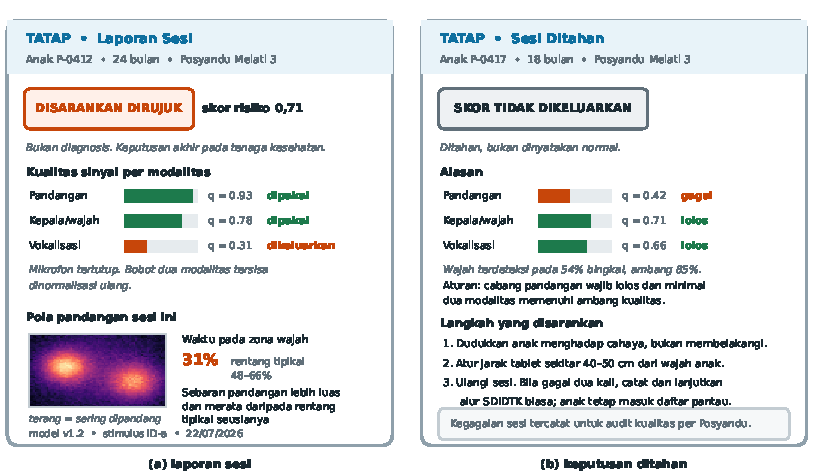
\includegraphics[width=0.80\textwidth]{../../figs/mockup.pdf}
\caption{Rancangan laporan \produk\ untuk kader. (a) Laporan sesi ketika cabang vokalisasi
dikeluarkan quality gate dan bobot dua modalitas tersisa dinormalisasi ulang. (b) Layar
penahanan keputusan ketika cabang pandangan gagal ambang kualitas. Angka pada gambar adalah
contoh ilustratif.}
\label{fig:mockup}
\end{figure}

\section*{Lampiran G. Rincian uji kelayakan pandangan}

Seluruh angka berikut berasal dari 547 citra dan 54 anak pada dataset \cite{carette2019}
dengan \textit{GroupKFold} lima lipatan per partisipan. Tabel~\ref{tab:model} menunjukkan
mengapa POC ini tidak menetapkan model produksi: urutan model berubah ketika metrik dihitung
pada unit anak, bukan unit rekaman. Regresi logistik, garis dasar yang dipilih sebelum hasil
dilihat, justru unggul pada unit anak terhadap model dengan AUC rekaman tertinggi.
\textit{Nested GroupKFold} memilih Naive Bayes pada kelima lipatan luar, sehingga estimasi
nested identik dengan estimasi biasa dan bias pemilihan model tidak menambah apa pun; namun
model dengan AUC anak tertinggi tidak pernah terpilih.

\begin{table}[H]
\centering
\small
\caption{Perbandingan lima model pada dua unit metrik. Nilai adalah hasil eksploratif pada
data publik, bukan klaim performa produk.}
\label{tab:model}
\begin{tabular}{@{}lcc@{}}
\toprule
\textbf{Model} & \textbf{AUC tingkat rekaman} & \textbf{AUC tingkat anak} \\
\midrule
Regresi logistik (pra-tetap) & 0,753 & 0,845 \\
SVM (RBF) & 0,733 & 0,849 \\
Naive Bayes & \textbf{0,775} & 0,834 \\
Random forest & 0,763 & \textbf{0,864} \\
Gradient boosting & 0,765 & 0,863 \\
\bottomrule
\end{tabular}
\end{table}

Dekomposisi penggelembungan pada Gambar~\ref{fig:bukti}c memakai regresi logistik dan 19
fitur identik di seluruh protokol, sehingga yang berubah hanya mekanisme evaluasi: \textbf{A}
0,816 augmentasi lalu pembagian acak per citra, \textbf{B} 0,797 augmentasi dikelompokkan per
citra sumber, \textbf{C} 0,748 augmentasi dikelompokkan per partisipan, \textbf{D} 0,753 tanpa
augmentasi dan dikelompokkan per partisipan. Selisih total 0,063 terurai menjadi 0,019 dari
kebocoran antarsalinan augmentasi (A--B) dan 0,048 dari tidak mengelompokkan per anak (B--C);
augmentasi sendiri, ketika pembagian sudah benar, menurunkan AUC 0,005 (C--D).

\end{document}
